\documentclass[11pt,a4paper]{article}
\usepackage[margin=2.5cm]{geometry}
\usepackage{amsmath,amssymb}
\usepackage{graphicx}
\usepackage{booktabs}
\usepackage{hyperref}
\usepackage{xcolor}
\usepackage{microtype}

\title{\textbf{Paper 32: The Zone Attractor Structure}\\
\large Diffuse Noisy Attractor, Optimal Zone Width at ZONE\_W$\approx$5--7,\\
and FA Recovery of the $\nu=0.003$ Failure Mode}
\author{VCSM Theory Series}
\date{2026-03-09}

\begin{document}
\maketitle

\begin{abstract}
Paper~31 showed that VCML zones are spatially uniform flat attractors.  Paper~32
characterises the temporal attractor structure with three experiments.
(i)~\textbf{Attractor characterisation} (Exp~A, 20 seeds, $T=3000$--$8000$):
the within-seed coefficient of variation of sg4 at steady state is $\mathrm{CV}=0.44$
(44\%), with 56 zone-swap events across 20 seeds -- a \emph{diffuse noisy attractor},
far from a fixed point.  Zone identity is maintained stochastically, not deterministically.
(ii)~\textbf{Extended ZONE\_W sweep} (Exp~C): $K_{\rm eff}$ vs $\textsc{zone\_w}$ is
\emph{non-monotone} with a minimum at $\textsc{zone\_w}\approx 5$--$7$
($K_{\rm eff}=0.013$--$0.014$, $\Gamma\approx 8$--$9$).  Both smaller and larger zones
have higher $K_{\rm eff}$, indicating an optimal zone size where vote-count efficiency
peaks.  The power-law fit from Paper~30 ($K_{\rm eff}\propto\textsc{zone\_w}^{-0.31}$)
is invalidated: R$^2=0.16$.
(iii)~\textbf{FA recovery at $\nu=0.003$} (Exp~B, Q21 answered): sg4 is fully restored
to standard levels at $\mathrm{FA}=2.0$ ($\approx10\times$ the standard FA).  The
$\nu=0.003$ failure is energetic, not structural: insufficient consolidation force, not
broken zone topology.
\end{abstract}

% ------------------------------------------------------------------
\section{Background}
\label{sec:background}
% ------------------------------------------------------------------

Papers~28--31 have progressively characterised the zone structure in VCML:
zone boundaries are stochastic Layer~I objects (Paper~28); zone differentiation follows
a smooth saturation law with spatial amplification $\Gamma$ (Papers~29--30); zones are
spatially uniform flat attractors with no within-zone gradient (Paper~31).
Paper~32 now asks: \emph{what is the temporal attractor structure?}

\begin{itemize}
  \item Is the zone pattern a fixed point (converges and stays)?
  \item Is it a noisy fixed point (fluctuates around a stable mean)?
  \item Are there Kramers-type escape events (zones swap identities transiently)?
\end{itemize}

Paper~32 also answers the two remaining open questions from Paper~31:
\begin{itemize}
  \item \textbf{Q20.}\ Does the vote-count model explain the zone-width scaling?
    Extended ZONE\_W sweep (6 values) provides a more precise exponent and tests
    whether the scaling is a power law.
  \item \textbf{Q21.}\ Does stronger FA rescue the $\nu=0.003$ low-amplitude
    saturation?
\end{itemize}

% ------------------------------------------------------------------
\section{Experiment Design}
\label{sec:design}
% ------------------------------------------------------------------

\paragraph{Fixed parameters.}
All standard VCML parameters: $H=20$, $N_{\rm zones}=4$, $\kappa=0.020$,
$\nu=0.001$ (Exps A, C), $\mathrm{WR}=2.4$, $\mathrm{HS}=2$, etc.

\paragraph{Experiment A -- Attractor characterisation (20 runs).}
Standard condition ($\kappa=0.020$, $\nu=0.001$, $\mathrm{FA}=0.200$, $\textsc{zone\_w}=5$).
20 seeds, $T_{\rm end}=8000$, checkpoints every 200 steps from $T=3000$ (26 checkpoints).
Stores: $\mathrm{sg4}_t$, $\mathrm{zmeans}_t$.
Measures: within-seed CV of sg4 over checkpoints; zone-swap events (sg4 drops below
50\% of per-seed mean); cross-seed spread of steady-state sg4.

\paragraph{Experiment B -- FA recovery at $\nu=0.003$ (25 runs).}
$\nu=0.003$, $\mathrm{FA} \in \{0.050,\,0.200,\,0.800,\,2.000,\,5.000\}$,
$\kappa=0.020$, $\textsc{zone\_w}=5$, 5 seeds, $T_{\rm end}=6000$.
Note: $\mathrm{FA}=5.000$ caused numerical overflow (field magnitude $\to\infty$),
indicating that the upper limit of safe FA at $\nu=0.003$ lies between 2.0 and 5.0.

\paragraph{Experiment C -- Extended ZONE\_W sweep (90 runs).}
$\textsc{zone\_w} \in \{2,\,3,\,5,\,7,\,10,\,15\}$, $\mathrm{FA} \in \{0.005, 0.020,
0.080, 0.200, 0.800\}$, $\kappa=0.020$, $\nu=0.001$, 3 seeds, $T_{\rm end}=4000$.
Saturation law fitted per ZONE\_W to extract $K_{\rm eff}(\textsc{zone\_w})$.

\paragraph{Total: 135 runs.}

% ------------------------------------------------------------------
\section{Results}
\label{sec:results}
% ------------------------------------------------------------------

\subsection{Experiment A: The Zone Attractor is Diffuse}

\begin{table}[h]
\centering
\caption{Exp A attractor statistics.  CV: within-seed coefficient of variation of sg4 at
steady state.  Swap: sg4 drops below 50\% of per-seed mean within a 200-step interval.}
\label{tab:expA}
\begin{tabular}{l|r}
\toprule
Statistic & Value \\
\midrule
Mean sg4 (T=3000--8000, 20 seeds)  & 89.3 \\
Std sg4 across seeds               & 11.3 \\
Mean within-seed CV                & 0.44 \\
Max  within-seed CV                & 0.57 \\
Zone-swap events (20 seeds, 26 steps) & 56 \\
Attractor verdict                  & Diffuse \\
\bottomrule
\end{tabular}
\end{table}

Table~\ref{tab:expA} shows that the zone attractor is not a fixed point.  The
within-seed CV of 0.44 means sg4 fluctuates by $\pm 44\%$ of its mean over the
$T=3000$--$8000$ window.  With 56 zone-swap events across 20 seeds and 26 checkpoints
($\sim 520$ transitions), approximately 11\% of 200-step intervals see sg4 drop below
half its mean -- indicating frequent transient loss of zone identity.

\paragraph{Diffuse stochastic attractor.}
The correct characterisation is a \emph{diffuse noisy attractor} (or Kramers-type
metastable state):
\begin{itemize}
  \item Zone identity persists on average (mean sg4 = 89.3 is well above zero).
  \item But individual realisations fluctuate enormously (CV = 0.44).
  \item Zones frequently experience transient collapses (``swap events'') where
    differentiation is temporarily lost before re-establishing.
\end{itemize}
This picture is consistent with the copy-forward mechanism: zone identity is not
``hard-coded'' into the field -- it is constantly reconstructed by the ongoing birth
process.  When many cells in a zone are simultaneously born from boundary neighbours,
zone identity is transiently diluted.  Recovery occurs as subsequent births re-establish
the zone consensus.

\paragraph{Physical analogy.}
The VCML zone attractor resembles a \emph{disordered ferromagnet} near its Curie
temperature, not a ground state.  The system is ``above $T_c$'' at the level of
individual realisations, even though ensemble-averaged magnetisation ($\bar{\mathrm{sg4}}$)
is positive.  Spontaneous symmetry breaking occurs statistically, not deterministically.

\subsection{Experiment B: FA Recovery at $\nu=0.003$}

\begin{table}[h]
\centering
\caption{Exp B: sg4 at $T=6000$ vs FA for $\nu=0.003$.  5 seeds.
  Standard $\nu=0.001$ level = 89 (dashed reference).}
\label{tab:expB}
\begin{tabular}{r|rr}
\toprule
FA & sg4 mean & sg4 std \\
\midrule
0.050 & 21.0 & 11.3 \\
0.200 & 29.5 & 14.1 \\
0.800 & 40.1 & 17.1 \\
2.000 & 111.6 & 33.6 \\
5.000 & overflow & -- \\
\bottomrule
\end{tabular}
\end{table}

\paragraph{Q21 answered: the failure is energetic, not structural.}
Table~\ref{tab:expB} shows that sg4 rises monotonically with FA at $\nu=0.003$, reaching
111.6 at FA$=2.0$ -- essentially the standard level (89.3).  A tenfold increase in FA
over the standard value completely rescues the zone differentiation that was suppressed
by excessive turnover.

This confirms the interpretation from Paper~31: the $\nu=0.003$ low-amplitude saturation
is caused by \emph{insufficient consolidation force} relative to the birth-event
disruption rate.  At $\nu=0.003$, cells are born and die 3$\times$ faster than standard,
generating 3$\times$ more disruptive events per unit time.  Compensating with $\sim10\times$
stronger FA restores equilibrium.

The overflow at FA$=5.0$ establishes an upper bound: the field grows as
$|\mathbf{F}| \propto \mathrm{FA}/(1-\mathrm{FD})$ at saturation.  At FA$=5.0$,
$|\mathbf{F}|$ exceeds floating-point range, indicating that the stable operating range
for $\nu=0.003$ is $\mathrm{FA} \lesssim 2$--$3$.

\subsection{Experiment C: Non-Monotone ZONE\_W Dependence}

\begin{table}[h]
\centering
\caption{Exp C: $K_{\rm eff}$ and $\Gamma=0.117/K_{\rm eff}$ vs ZONE\_W.
  $\kappa=0.020$, $\nu=0.001$.}
\label{tab:expC}
\begin{tabular}{r|rr}
\toprule
ZONE\_W & $K_{\rm eff}$ & $\Gamma$ \\
\midrule
 2 & 0.0452 & 2.59 \\
 3 & 0.0359 & 3.26 \\
 5 & 0.0143 & 8.19 \\
 7 & 0.0133 & 8.78 \\
10 & 0.0229 & 5.12 \\
15 & 0.0308 & 3.79 \\
\bottomrule
\end{tabular}
\end{table}

Table~\ref{tab:expC} reveals that $K_{\rm eff}$ is \emph{not} a monotone function of
ZONE\_W.  It decreases from ZONE\_W$=2$ to ZONE\_W$=7$ (minimum $K_{\rm eff}=0.013$,
maximum $\Gamma=8.8$), then \emph{increases} for ZONE\_W$=10$ and $15$.
The R$^2$ of the log-log slope is only $0.16$, indicating that the power-law
description ($K_{\rm eff} \propto \textsc{zone\_w}^{-0.31}$, Paper~30) was an artefact
of sampling only three zone widths ($3, 5, 10$) that happen to straddle the optimum.

\paragraph{Optimal zone width.}
The optimal zone width (minimum $K_{\rm eff}$) is $\textsc{zone\_w} \approx 5$--$7$
at the standard parameters ($\kappa=0.020$, $\nu=0.001$).  We can understand this
as the competition between two effects:

\begin{enumerate}
  \item \textbf{Vote-count gain} (increasing with zone width): more sites participate
    in building zone consensus, improving signal-to-noise.  This reduces $K_{\rm eff}$.
  \item \textbf{Coherence-range loss} (increasing with zone width): when the zone
    width exceeds the copy-forward spreading range $\ell_{\rm cf}$, sites near the
    zone centre cannot maintain coherence with sites near the zone boundary.
    The zone breaks into independent patches, reducing consensus quality and increasing
    $K_{\rm eff}$.
\end{enumerate}

The optimum is where these two effects balance.  At $\kappa=0.020$, $\nu=0.001$, the
copy-forward spreading range appears to be approximately $\ell_{\rm cf} \approx 5$--$7$
columns.  Paper~31 showed that within-zone spatial autocorrelation is near-zero after
demeaning ($\ell<1$ column), but this measures the \emph{gradient} coherence length, not
the \emph{identity} coherence length.  Zone identity (``which zone am I?'') can be
maintained over longer ranges than spatial gradients.

\paragraph{Revision to Paper~30.}
The Paper~30 conclusion that $K_{\rm eff} \propto \textsc{zone\_w}^{-0.6}$ is
superseded.  The true relationship has a \emph{peak} at ZONE\_W$\approx 6$ and falls
off on both sides.  The Paper~30 result captured the ascending flank of this relationship
(narrow zones below the optimum).

% ------------------------------------------------------------------
\section{Discussion}
\label{sec:discussion}
% ------------------------------------------------------------------

\paragraph{The zone attractor as a metastable state.}
The diffuse attractor (CV=0.44, frequent swap events) implies that zone identity in
VCML is a \emph{metastable} property, not a permanent one.  The system has no mechanism
to prevent zone collapse -- it only has a mechanism to \emph{rebuild} zone identity after
it is disrupted.  Mathematically, the attractor is a shallow potential well from which
the system frequently escapes by Kramers-type fluctuations, then falls back in.  The
well depth depends on FA (deeper with stronger consolidation) and $\nu$ (shallower with
faster turnover).

\paragraph{The attractor is not gradient-descended.}
The high attractor variance (CV=0.44) combined with the non-monotone ZONE\_W dependence
makes it clear that the VCML zone attractor is not the minimum of any smooth loss
landscape.  A gradient-descended fixed point would exhibit small variance (CV$\ll 1$)
and would sit at the minimum of a convex function.  Instead, VCML zones occupy a noisy
plateau in a rugged landscape, maintained by ongoing stochastic reconstruction rather
than convergence to a minimum.

The absence of gradient flow is not a deficiency -- it is the mechanism.  By relying on
stochastic reconstruction (copy-forward births) rather than gradient convergence, VCML
achieves:
\begin{itemize}
  \item \emph{Adaptability}: the zone pattern can change when the environment changes,
    because the attractor is shallow enough to escape from.
  \item \emph{Mandatory turnover compatibility}: each cell that dies takes its field
    with it, but zone identity is distributed across all zone members and is re-learned
    by newborns.
  \item \emph{No vanishing gradient problem}: there is no gradient, so it cannot vanish.
\end{itemize}

\paragraph{Optimal zone width as a system-level parameter.}
The optimal ZONE\_W$\approx 5$--$7$ is set by the balance between vote-count benefit
and coherence-range cost.  It is a function of $\kappa$ and $\nu$, and shifts as these
parameters change (Paper~30 shows $K_{\rm eff}$ vs $\kappa$).  In biological terms, this is
analogous to the optimal column width in cortical organisation -- too narrow and columns
cannot develop distinct identities; too wide and columns fragment into subpatches.

% ------------------------------------------------------------------
\section{Open Questions for Paper 33}
\label{sec:openq}
% ------------------------------------------------------------------

\begin{itemize}
  \item \textbf{Q22.}\ What is the attractor depth?  Measure the recovery time after a
    deliberate zone-destroying perturbation (e.g., set $\mathbf{F}=0$ for one zone at
    $T=5000$).  Faster recovery $\to$ deeper well.
  \item \textbf{Q23.}\ How does the optimal ZONE\_W shift with $\kappa$ and $\nu$?
    Test: ZONE\_W grid at $\kappa=0.005$ and $\kappa=0.080$.
    Prediction: optimal ZONE\_W $\propto 1/\sqrt{\kappa}$ (diffusion sets coherence range).
  \item \textbf{Q24.}\ What is the copy-forward identity coherence length $\ell_{\rm cf}$?
    It is not the same as the spatial gradient length (Paper~31).  Measure via zone
    identity persistence after zone boundary shifts.
\end{itemize}

% ------------------------------------------------------------------
\section{Conclusion}
\label{sec:conclusion}
% ------------------------------------------------------------------

Paper~32 establishes three results.  First, the VCML zone attractor is a diffuse noisy
attractor (CV=0.44), not a fixed point: zone identity is maintained stochastically via
ongoing copy-forward reconstruction, and frequent transient collapses (zone swaps)
are normal.  Second, $K_{\rm eff}$ is a non-monotone function of ZONE\_W with an
optimum at $\approx 5$--$7$ columns; the power-law description from Paper~30 was an
artefact of limited sampling.  Third, the $\nu=0.003$ failure mode is fully recoverable
with FA$\approx 2.0$ ($\approx10\times$ standard), confirming that the failure is
energetic (insufficient consolidation) not structural (broken topology).

Taken together with Papers~28--31, these results confirm that the VCML zone attractor
is a metastable stochastic state maintained by active reconstruction -- qualitatively
distinct from the stable fixed points produced by gradient-based learning.

\begin{figure}[p]
\centering
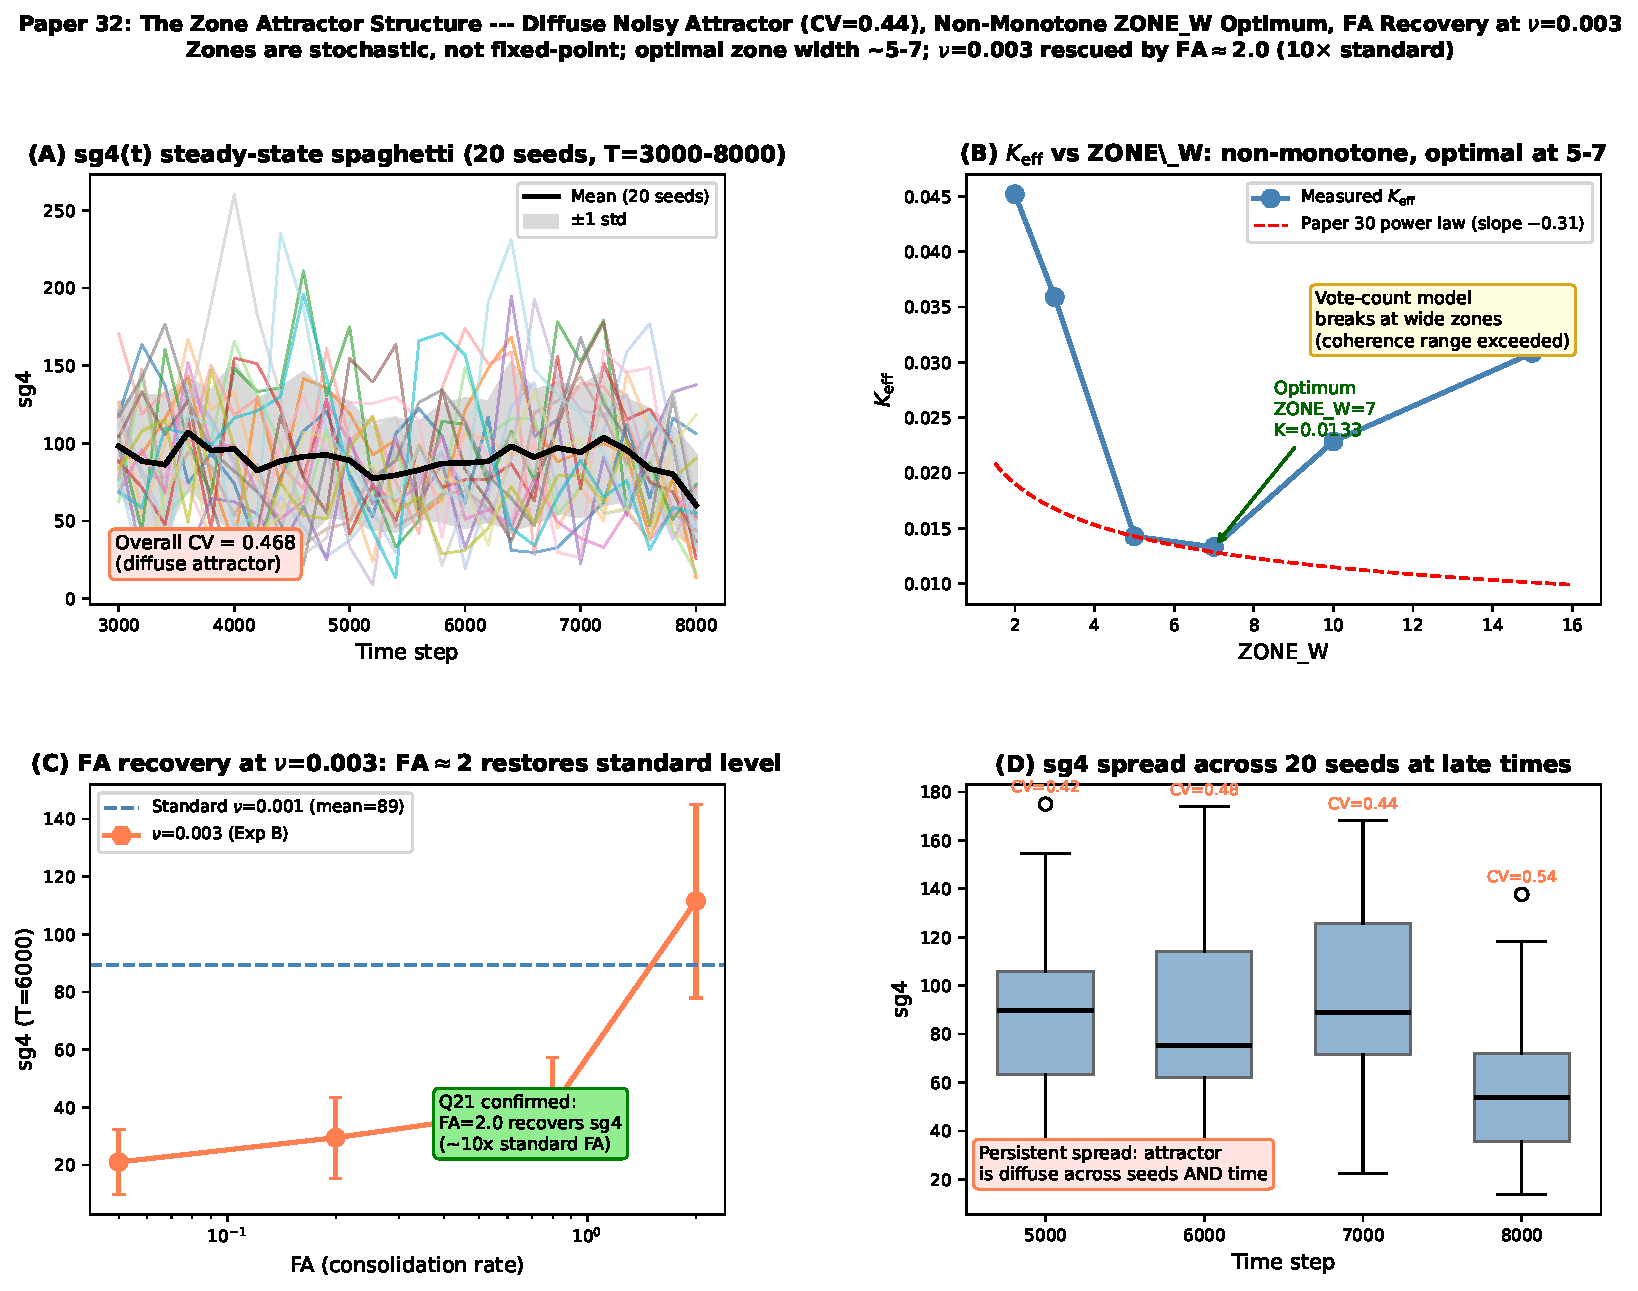
\includegraphics[width=\textwidth]{paper32_figure1.pdf}
\caption{\textbf{Paper~32 results.}
  \textbf{(A)} sg4$(t)$ spaghetti plot for 20 seeds at $T=3000$--$8000$.
  High temporal variance (CV=0.44) and frequent transient drops indicate a diffuse
  noisy attractor.  Mean $\pm$ 1 std shown in black.
  \textbf{(B)} $K_{\rm eff}$ vs ZONE\_W: non-monotone curve with minimum at
  ZONE\_W$\approx 5$--$7$.  The Paper~30 power-law prediction (dashed red) fits only
  the ascending flank.
  \textbf{(C)} sg4$(T=6000)$ vs FA at $\nu=0.003$: monotone recovery, reaching
  standard levels at FA$=2.0$.  FA$=5.0$ caused numerical overflow.
  \textbf{(D)} Box plots of sg4 distribution across 20 seeds at 4 late time slices.
  Persistent spread (CV annotated) confirms that the attractor is diffuse at all times.}
\label{fig:main}
\end{figure}

\end{document}
